\documentclass[fleqn,11pt,openany]{book}

% These two need to be set before including scirun style package
\title{Seg3D Basic Functionality}
\author{Jess Tate}

% INCLUDE SCI STYLE DOCUMENT
\usepackage{seg3d}
\usepackage{marvosym}

\begin{document}

%% starting from SCIRun Doc wiki
%% http://software.sci.utah.edu/SCIRunDocs/index.php/CIBC:Documentation:SCIRun:Tutorial:BioPSE


% CREATE TITLE PAGE --------------------------------------------------
\maketitle

% CHAPTERS ---------------------------------------------------------------

\chapter{Overview}

\begin{introduction}

This document is meant as a basic reference and walkthrough of the Seg3D layout and functionality.  

\end{introduction}

\section{Software requirements}

\subsection{Seg3D 2.1}

Seg3D is distributed as a binary download for Linux, Windows, and OS X. Please visit the SCI software portal ({http://software.sci.utah.edu} ) to download the latest Seg3D binary. Any version of 2.0 or higher will do. 

%---------------------------------------------


\chapter{Welcome Screen}

%\begin{figure}
%\scalebox{0.3}{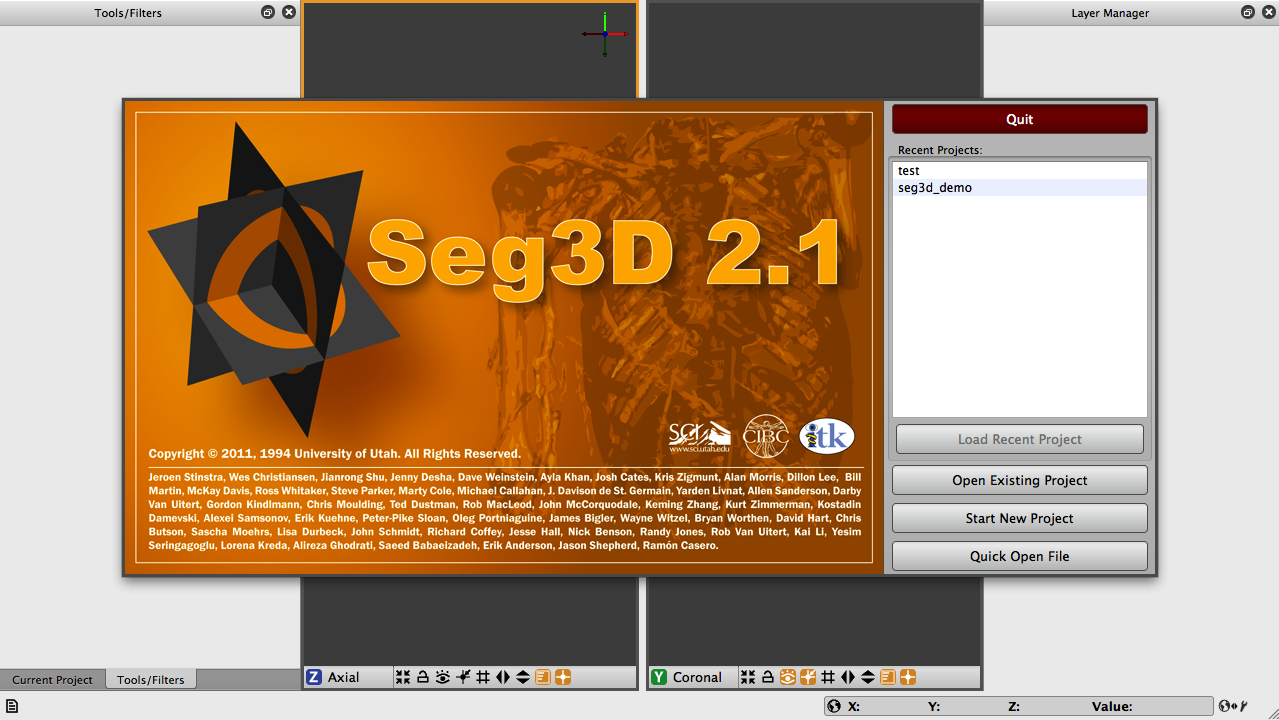
\includegraphics{Seg3DTutorial_figures/welcome_screen.png}}
%\caption{Seg3D welcome screen}\label{fig:welcome}
%\end{figure}

\chapter{Seg3D Viewer}

\begin{introduction}

\end{introduction}

\section{2D Slice Viewer}

\section{3D Volume Viewer}

\section{Viewing Options}

\chapter{Seg3D Windows}

\begin{introduction}

\end{introduction}

\section{Project Window}

\section{Tools Window}

\section{Layer Manager Window}

\section{Volume View Window}

\section{Provenance Window}

\section{Controller Window}

\section{Python Console}

\chapter{Basic Program Functions}

\begin{introduction}

\end{introduction}

\section{File}

\subsection{New Project}

\subsection{Open Project}

\subsection{etc.}

\section{Edit}

\section{Help}

\section{Preferences}

\chapter{Tools \& Filters}

\begin{introduction}

\end{introduction}

\section{Tools}

\subsection{Copy/Paste}

\subsection{Crop}

\subsection{etc.}

\section{Mask Filters}

\subsection{etc.}

\section{Data Filters}

\subsection{etc.}

\section{Advanced Filters}

\subsection{etc.}

\end{document}

